\documentclass{article}

\usepackage{graphicx} % Required for inserting images

\usepackage{subfigure}

\usepackage{subcaption}

\usepackage{float}

\usepackage{siunitx}

\usepackage{geometry}

\geometry{legalpaper, portrait, margin=1in}

\usepackage{mathtools}
\DeclarePairedDelimiter\bra{\langle}{\rvert}
\DeclarePairedDelimiter\ket{\lvert}{\rangle}
\DeclarePairedDelimiterX\braket[2]{\langle}{\rangle}{#1\,\delimsize\vert\,\mathopen{}#2}

\title{Rb}
\author{Anas Roumeih}
\date{June 2024}

\begin{document}

\maketitle

\section{Introduction}
\subsection{Natural line width}
The line of a resonant frequency has a finite width and is not infinitely narrow, regardless of any thermal effects. This broadening is due to the Heisenberg uncertainty principle, which can be expressed as: 
\begin{equation}
    \Delta E\Delta t \sim \hbar
\end{equation}
Molecules in an excited state can be described by a harmonic oscillator and the energy loss due to radiation is equivalent to an attenuation of this oscillation. A solution to such system is periodic, and hence separable into Fourier components. The intensity measure is proportional to the squared amplitude of the Fourier transform of our oscillating solution [demtroder laser spec 1]: 
\begin{equation}
    I(\omega-\omega_0) = I_0\frac{\gamma/2\pi}{(\omega-\omega_0)^2+(\gamma/2)^2}
\end{equation}

This expression for the intensity yields a Lorentzian profile, its full-width-at-half-maximum (FWHM) is the natural line width $\delta\omega_n = \gamma$. An electron stays in an excited state $E$ for time $\Delta t$ before transitioning back to a ground state. According to the uncertainty principle, the uncertainty in the energy is $\Delta E\sim \hbar/\Delta t$ and thus: 
\begin{equation}
    \Delta\omega = \frac{1}{\Delta t}
\end{equation}
We identify $\Delta\omega$ with $\delta\omega_n$ and $\Delta t$ with $\tau$ \textit{the lifetime of the state}, which is the time after which the emitted intensity has dropped by $1/e$ of its initial value [1]. So now we can relate the lifetime of an excited state to the FWHM of the radiation peak. 
\subsection{Doppler Broadening}
Doppler broadening happens due to the thermal motion of particles. The velocity distribution of the particles is described by Maxwell-Boltzmann statistics. A molecule emitting moving with a velocity $v$ with respect to a non-moving observer, the observer will see a frequency $\omega = \omega_0 + \vec{k} \cdot \vec{v}$. Assuming $\vec{k}$ points in the z-direction we get: 
\begin{equation}
    \omega = \omega_0(1+\frac{v_z}{c})
\end{equation}
For a constant density of states and an ideal gas, the velocity z-component has the probability distribution: 
\begin{equation}
    p\left(v_z\right) \mathrm{d} v_z=\sqrt{\frac{m}{2 k_B T \pi}} e^{\frac{-m v_z^2}{2k_BT}}=\frac{1}{v_p \sqrt{\pi}} e^{-\left(\frac{v_z}{v_p}\right)^2} \mathrm{~d} v_z  
\end{equation}
where $v_p$ is the most probable velocity. Which relates to the number of molecules in the level $E_i$ per unit volume with a velocity component between $v_z$ and $v_z+\mathrm{d} v_z$ by: 
\begin{equation}
    n_i\left(v_z\right) \mathrm{d} v_z=\frac{N_i}{v_{\mathrm{p}} \sqrt{\pi}} e^{-\left(v z / v_{\mathrm{p}}\right)^2} \mathrm{~d} v_z,
\end{equation}
Where $N_i=\int n_i\left(v_z\right) \mathrm{d} v_z$ is the density of all molecules in the level $E_i$. Since that we work with frequencies in the experiment, it makes sense to make the substitution $v_z = c(\frac{\omega}{\omega_0}-1)$ with $\mathrm{d}v_z = \frac{c}{\omega_0}\mathrm{d}\omega$ yielding: 
\begin{equation}
    n_i(\omega) \mathrm{d} \omega=\frac{N_i}{v_p \sqrt{\pi}} \frac{c}{\omega_0} e^{-c^2\left(\frac{\omega-\omega_0}{v_p \omega_0}\right)^2}\mathrm{d}\omega
\end{equation}
And since the intensity is proportional to $n_i(\omega)$ we get: 
\begin{equation}
    I(\omega) =I\left(\omega_0\right) e^{-\left(\frac{\omega-\omega_0}{\omega_0 v_p/c} \right)^2}
\end{equation}
Which is a Gaussian distribution, with a FWHM: 
\begin{equation}
    \delta \omega_D =\frac{\omega_0}{c} \sqrt{\frac{k_B T \ln(2)}{m}}
\end{equation}
Where $M$ is the molar mass of the molecules. It is worth mentioning that this FWHM is much higher than the natural line width, as the broadening grows proportionally to the eigenfrequency [1].


Since every radiating transition in the Doppler-Gaussian profile has a Lorentzian profile at different frequencies. A Voigt profile is constructed, which is a convolution of the two profiles mentioned. 
\begin{equation}    
    I\left(\omega-\omega^{\prime}\right)=I_0 \int\left(\omega-\omega^{\prime}\right) n\left(v_z\right) d v_z
\end{equation}

\begin{figure}
    \centering 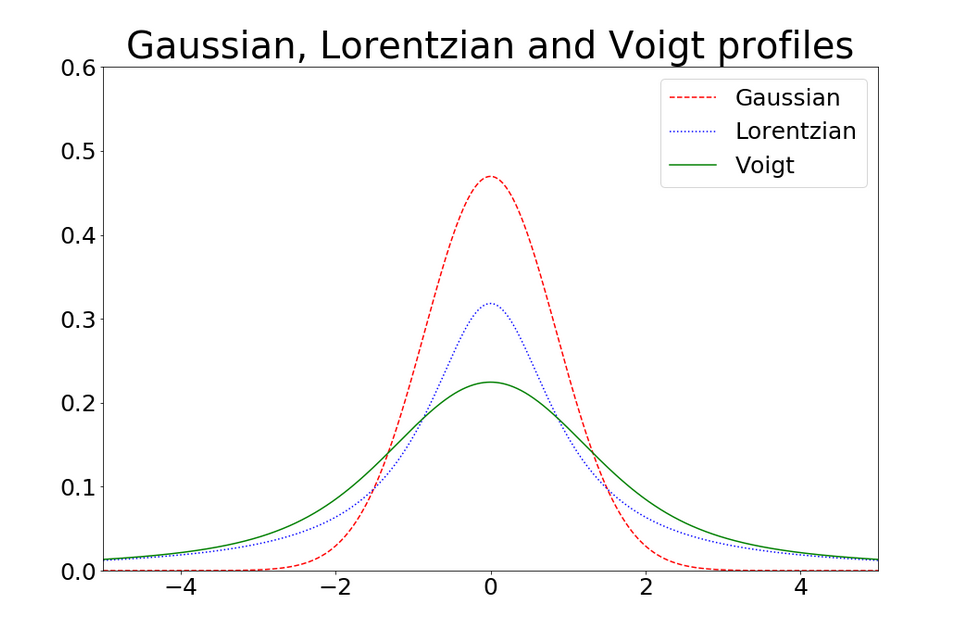
\includegraphics[width=0.5\linewidth]{1.png}
    \caption{The three profiles}
    \label{fig:enter-label}
\end{figure}

\subsection{Homogeneous and inhomogeneous line broadening}

A transition's spectral profile is considered \textit{homogeneous} if every molecule or atom in state $\ket{i}$ has an equal probability of transitioning to state $\ket{k}$. The probability of emitting radiation is then: 
\begin{equation}
   P(\omega) = A_{ki}g(\omega-\omega_0) 
\end{equation}
Where $A_{ki}$ are the Einstein coefficients of spontaneous emission and $g(\omega-\omega_0)$ is a normalized Lorentzian profile. 

\subsection{Linear absorption spectroscopy} 
Linear absorption spectroscopy is a technique in which an atomic sample (in our case, the rubidium gas), is examined while a tunable single-laser mode laser beam shines at the sample. The frequency of the laser is varied and the intensity pattern of the transmitted beam is measured with a photodiode. 

This method is significantly hindered by the Doppler broadening of absorption lines. For instance, the twelve permissible hyperfine transitions of Rb cannot be individually distinguished using this technique. This is because the Doppler width (approximately 10 GHz) is substantially larger than the frequency gap between the absorption lines, resulting in their overlap. To address this issue, the method of \textit{saturation absorption spectroscopy} is employed.

\subsection{Saturation absorption spectroscopy}

The method of saturation absorption spectroscopy makes it possible to completely eliminate the Doppler background by measuring the difference between the normal and saturated absorption. Thus providing a clear resolution of all the transitions relevant in our experiment. 

In this approach, the beam is divided into two beams with different intensities: a weak probe beam (about 4-5\% of the total intensity) and a pump beam with the rest of the intensity. Both beams strike the gas cell in an opposite direction, and the signal from the probe beam is as a function of the laser frequency.
\\
Consider an atom with two levels and a resonance frequency $\omega_0$. If only the probe beam is used to study the gas cell, we will get the absorption lines we expect to get from linear absorption spectroscopy (with lower intensity). Introducing the pump beam will lead to a very narrow dip in the probe beam signal at the resonance frequency $\omega_0$ (see figure 2). Which can be understood as follows. Atoms with zero velocity component along the z-direction ($v_z = 0$) see both beams as having the same frequency (no Doppler effect). However if an atom happens to have a velocity component along the z-direction, it will see  a shifted frequency of the beams. If the atom is moving to the left (see figure) it will see the probe and pump beams as blue-shifted and red-shifted, respectively. If the atom is moving to the right, the opposite will happen. The pump beam's high intensity will excite all atoms with velocity $v_z = \frac{\omega_L - \omega_0}{\omega_0}c$, where $\omega_L$ is the frequency of the beam. Which will cause absorption for all the atoms with velocity $-v_z$ of the probe beam. Hence, the absorption signal will be the same as in the case of linear absorption spectroscopy. However, if the laser's frequency matches the resonance frequency ($\omega_L = \omega_0$), the atoms with $v_z =0$ will be excited by the high intensity of the pump beam and the ground state will be depleted. Consequently, the absorption rate for the probe beam decreases, leading to a narrow dip with a Lorentzian shape (as the Doppler shift is not present at resonance). This phenomenon is referred to as \textit{hole burning}, and the dips are known as \textit{Lamb dips}.
\begin{figure}[H]
    \centering
    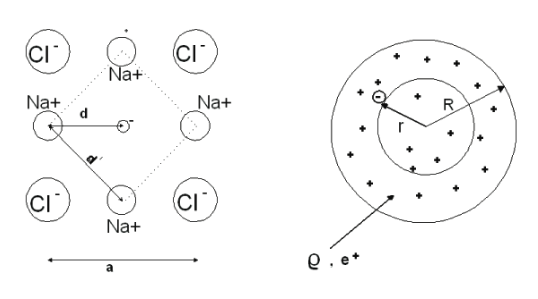
\includegraphics[width=0.5\linewidth]{3.png}
    \caption{Saturation peak in the Doppler-broadened profile of a two-level atom.}
    \label{fig:enter-label}
\end{figure}
\begin{figure}[H]
    \centering
    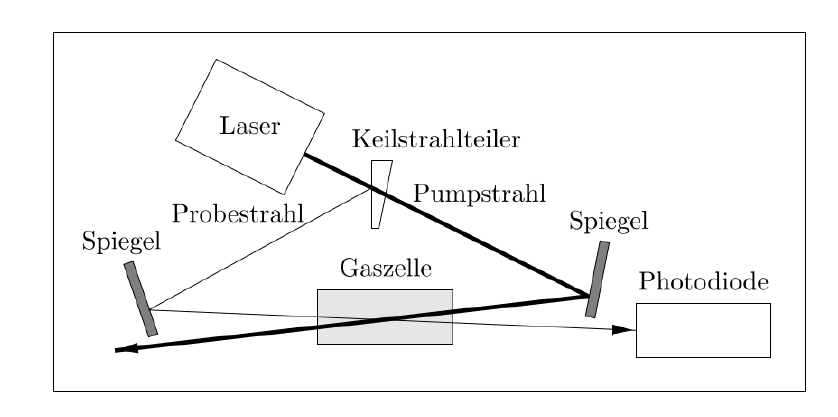
\includegraphics[width=0.5\linewidth]{2.png}
    \caption{Diagram of the basic setup of saturation absorption spectroscopy.}
    \label{fig:enter-label}
\end{figure}

Now consider a multi-level system. The Doppler broadened absorption lines will have more dips since more transitions can take place and we observe the phenomenon of \textit{cross-over signals}.
Consider a system with three levels, denoted as $N=\{0, 1, 2\}$. If the pump beam’s frequency resonates with either of the transitions $\omega_{01}$ and $\omega_{02}$, two saturation peaks will appear. This is due to the reduction of atoms with a velocity of $v_z = 0$. When the laser frequency is at the average of these frequencies 
\begin{equation}
    \omega_{12} = \frac{\omega_{01}+\omega_{02}}{2}
\end{equation}
the atoms that have a velocity 
\begin{equation}
    v_z = \frac{(\omega_{12}-\omega_{01})c}{\omega_{12}} = \frac{(\omega_{02}-\omega_{01})c}{2\omega_{12}} 
\end{equation}
are excited by the frequency $\omega_{02}$ from the pump beam and the frequency $\omega{01}$ from the probe beam. In a similar fashion, the atoms with velocity 
\begin{equation}
   - v_z = \frac{(\omega_{12}-\omega_{02})c}{\omega_{12}} 
\end{equation}
which gives: 
\begin{equation}
    v_z = \frac{(\omega_{02}-\omega_{01})c}{2\omega_{12}}
\end{equation}
will be excited by the frequency $\omega_{01}$ from the pump beam and the frequency $\omega_{02}$ from the probe beam. Since most atoms are now excited by the pump beam, they are unable to absorb the frequency of the probe beam which manifests as a third dip which is larger than the saturation peaks (Figure 4). This dip is what we call a cross-over peak.

\begin{figure}[H]
    \centering
    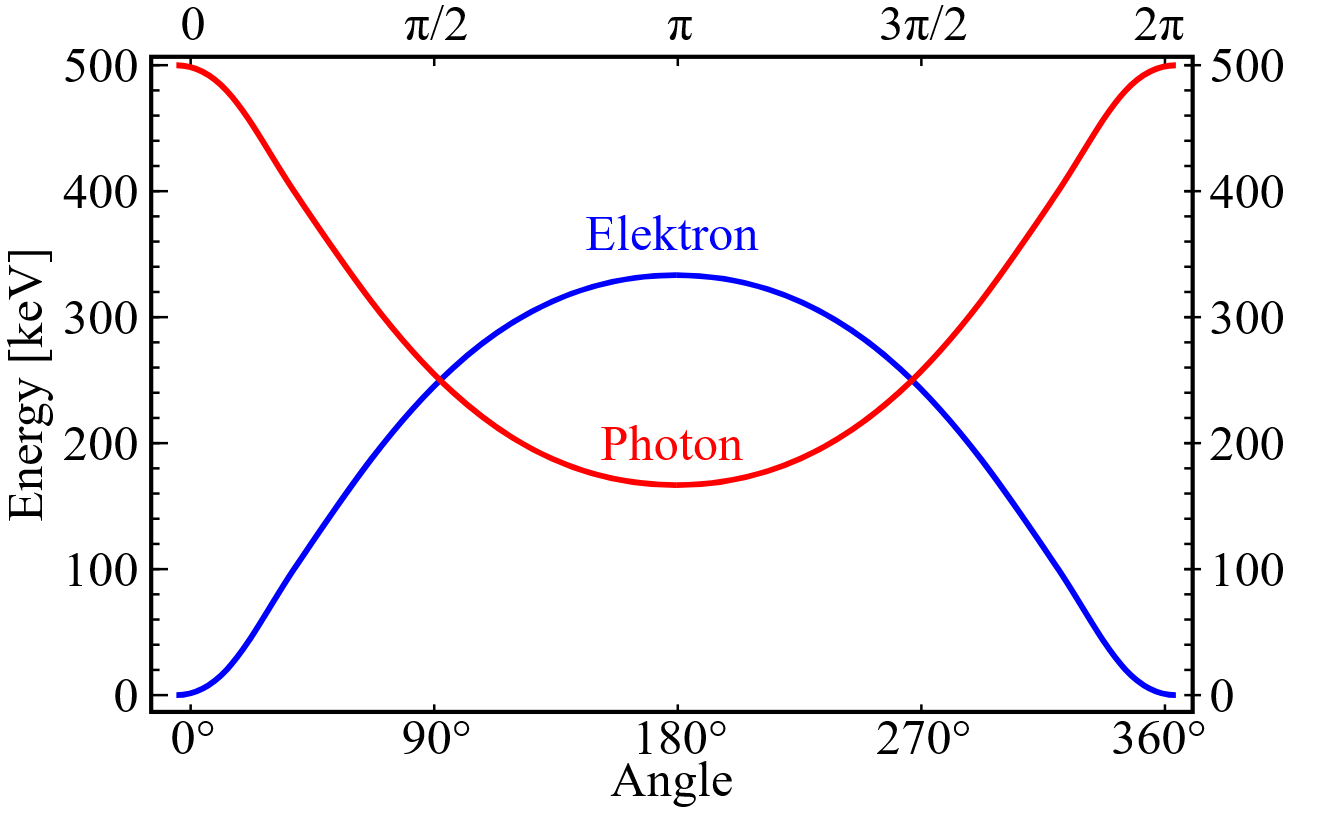
\includegraphics[width=0.5\linewidth]{4.png}
    \caption{Saturation peaks and crossover signal in the spectrum of a atoms with a three-level systems.[idk]}
    \label{fig:enter-label}
\end{figure}

In simpler terms, if two molecular transitions with resonant frequencies $\omega_1$ and $\omega_2$ share a common lower or upper level and overlap within their Doppler width $\delta\omega_D$ (i.e. $|{\omega_1 - \omega_2}| <\delta\omega_D$), a cross-over signal will appear at the frequency $\omega = (\omega_1 + \omega_2)/2$.

\subsection{Fine structure of Rubidium}
Rubidium is an alkali metal that occurs in nature with a mixture of about 72\% $^{85}Rb$ and 28\% $^{87}Rb$. In our experiment, rubidium is present as a gas in a gas cell. This is easily achievable at room temperature since it has a low melting point (around $\SI{39}{\celsius}$) and a boiling point of $\SI{688}{\celsius}$. It is important to note that in alkali metals, all energy levels are filled in the ground state except for the highest one, which is singly occupied. The electron configuration for rubidium in the ground state is $5s^1$. 
\\
Fine structure occurs due to the interaction between electron spin and orbital angular momentum. An extra contribution in the Hamiltonian causes a splitting of the excited states. This contribution is proportional to the product $\vec{S}\cdot\vec{L}$. New quantum numbers are introduced $j$ and $j_z$, which are the eigenvalues of the operator $\vec{J}= \vec{S}+\vec{L}$ and its projection onto the z-axis $\vec{J}_z$ respectively. This is because the operators $\vec{S}$ and $\vec{J}$ don't commute with the Hamiltonian anymore. However, the newly defined total angular momentum $\vec{J}$ does. This definition yields: 
\begin{equation}
    |l-s| \leq j \leq|l+s|
\end{equation}
In spectroscopic notation, the ground state of rubidium is $5^2S_{3/2}$ (i.e. $l=0$,$s=1/2$,$j = 1/2$). The splitting of the first excited state of rubidium is interpreted as having two values of $j$ which are $j =1/2$ and $j =3/2$, resulting in the two states $5^2P_{1/2}$ and $5^2P_{3/2}$, respectively. Hence, two different transitions can take place, termed the $D_1$ and $D_2$ lines: 
\begin{equation}
    \begin{aligned}
& D_1: 5^2 S_{\frac{1}{2}} \Rightarrow 5^2 P_{\frac{1}{2}} \nu_{1}=\SI{377.1}{THz} \\
& D_2: 5^2 S_{\frac{1}{2}} \Rightarrow 5^2 P_{\frac{3}{2}} \nu_{2}=\SI{384.2}{THz} 
\end{aligned}
\end{equation}
In our experiment, we work with the $D_2$ line. 

\subsection{Hyperfine structure of Rubidium}

Since nuclei are made of neutrons and protons, they have an intrinsic angular momentum $\vec{I}$. The interaction between $\vec{I}$ and $\vec{J}$ leads to further splitting in the same spirit as spin-orbit coupling. A new operator is defined as $\vec{F} = \vec{I}+\vec{J}$ with an eigenvalue $f$ taking the values $|j-i| \leq f \leq|j+i|$. The interaction strength and hence the splitting will be different between the two isotopes of rubidium that we are working with. The energy levels that result from the splitting are: 
\begin{equation}
    \begin{gathered}
\text { ground state: } \\
{ }^{85} R b: j=\frac{1}{2} \Rightarrow i=\frac{3}{2}, f=1,2 \\
{ }^{87} R b: j=\frac{1}{2} \Rightarrow i=\frac{5}{2}, f=2,3 \\
\text { excited state: } \\
{ }^{85} R b: j=\frac{1}{2} \Rightarrow i=\frac{3}{2}, f=1,2 \\
{ }^{85} R b: j=\frac{3}{2} \Rightarrow i=\frac{3}{2}, f=0,3 \\
{ }^{87} R b: j=\frac{1}{2} \Rightarrow i=\frac{5}{2}, f=2,3 \\
{ }^{87} R b: j=\frac{3}{2} \Rightarrow i=\frac{5}{2}, f=1,4
\end{gathered}
\end{equation}

\subsection{Semiconductor basics}
Semiconductors are solids that have a conductivity between that of a conductor and an insulator. Their energy levels sit close to each other in what is known as 'band structure'. The lower energy band is known as the valence band while the higher energy one is the conduction band. There is an energy gap (the \textit{band gap)} between the two bands where no energy level is allowed. At the middle of the band gap lays the Fermi level, which at absolute zero, separates the fully empty conduction band from the fully occupied valence band. The position of the Fermi level affects the conductivity of the semiconductor, and it can be controlled with the method of \textit{doping}.
\begin{figure}[H]
    \centering
    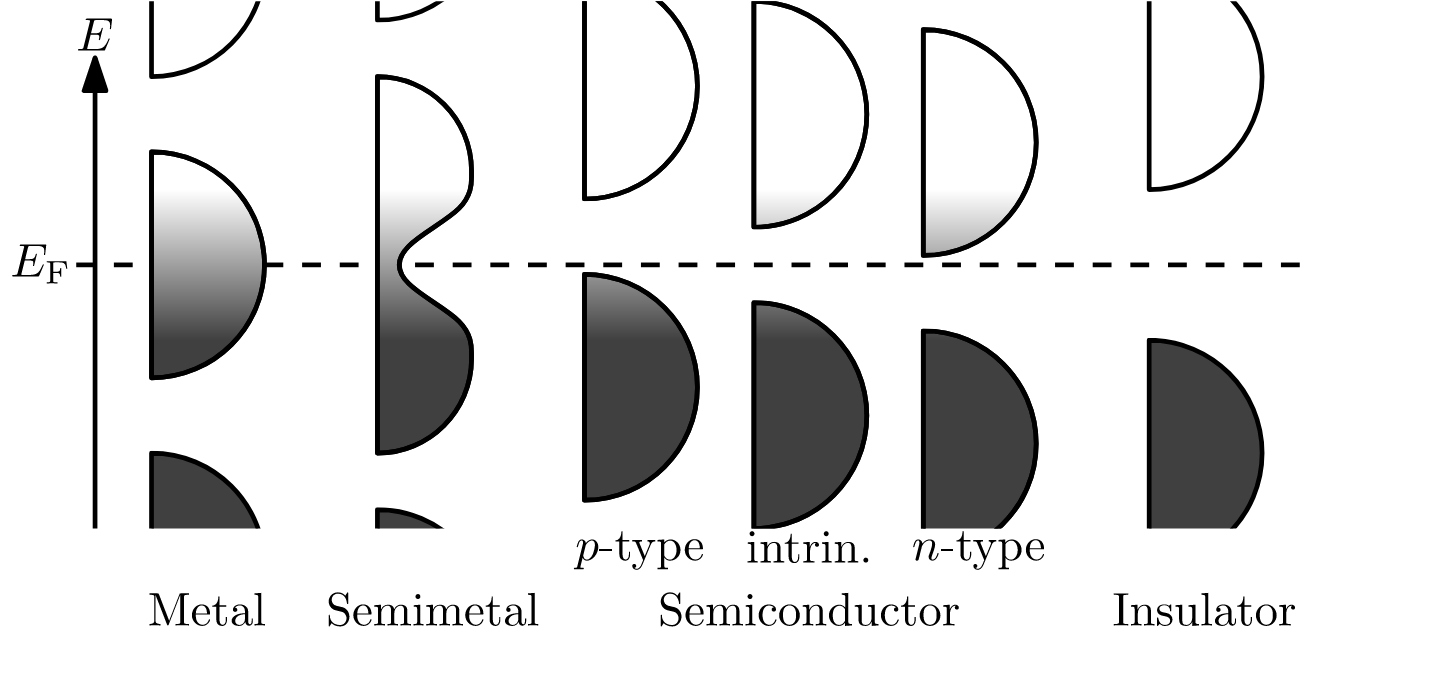
\includegraphics[width=0.5\linewidth]{wiki2.png}
    \caption{Position of Fermi level in different materials \cite{wikipediacontributors_2019_semiconductor}}
    \label{fig:enter-label}
\end{figure}


\subsection{Doping}
Doping is a technique that involves substituting a semiconductor lattice atom with another atom that has a different number of valence electrons. There are two kind of doping, n-doping and p-doping. P-doping involves replacing an atom from the lattice by another atom that has fewer valence electrons. In n-doping the impurity has more valence electrons than the lattice atoms. P-doping introduces a 'hole', which is an absence of an electron and is equivalent to a positive charge. Doping is useful because it lets us modify the conductivity of a semi-conductor. For example, in n-doping, the Fermi level is shifted and becomes closer to the conduction band, making it possible for an electron to jump to the conduction band via thermal excitations. This leads to an increase in the density of free charge carriers and hence the conductivity of the lattice. 
\begin{figure}[H]
    \centering
    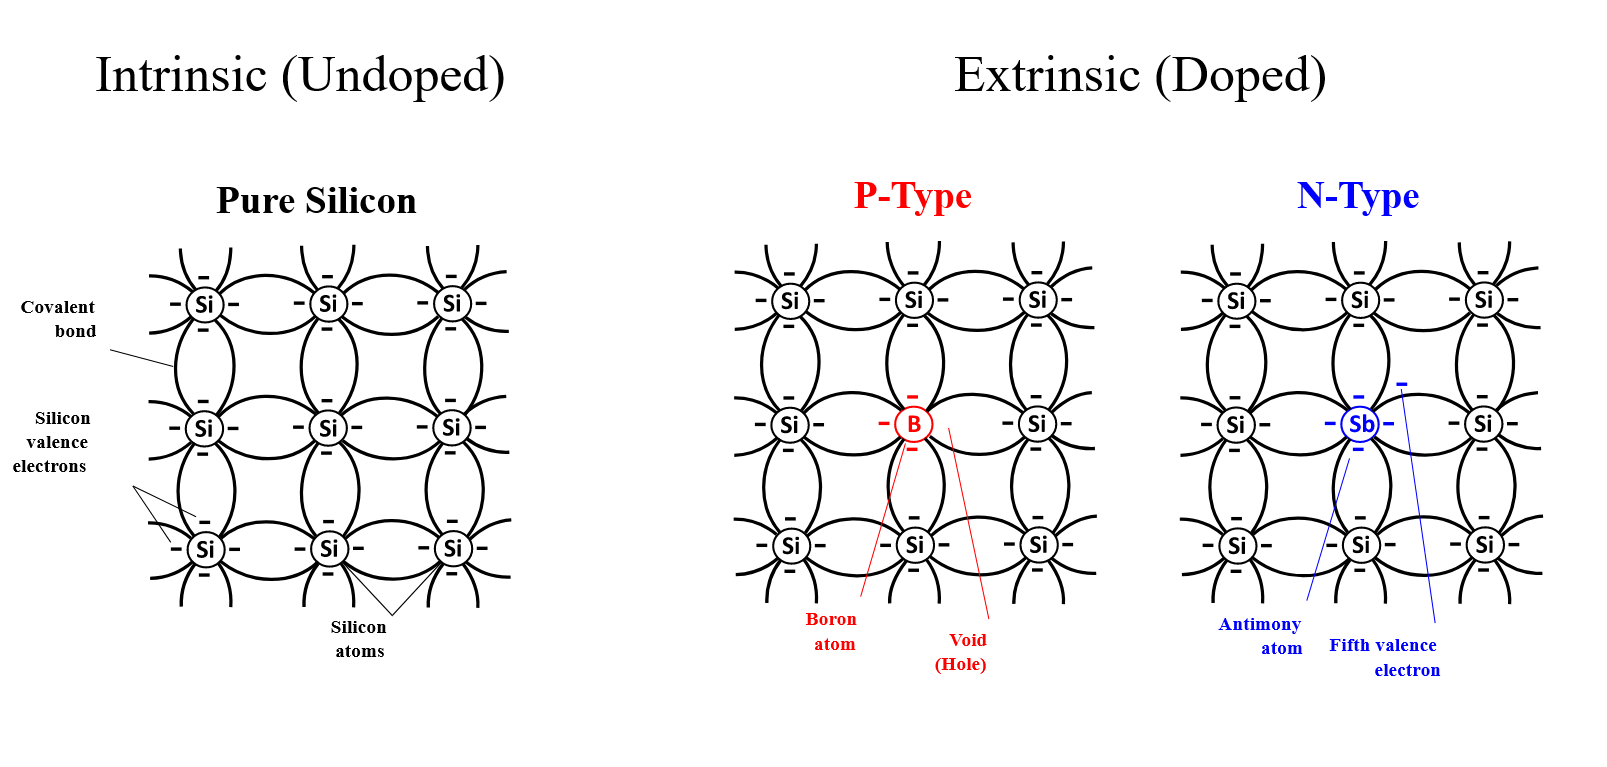
\includegraphics[width=0.5\linewidth]{wiki1.png}
    \caption{Doping of a pure silicon array. Silicon based intrinsic semiconductor becomes extrinsic when impurities such as Boron and Antimony are introduced. \cite{wikipediacontributors_2019_doping}}
    \label{fig:enter-label}
\end{figure}

\subsection{The p-n junction}
A p-n junction is a combination of a p- and n- doped semiconductors. When the two regions come in contact, a recombination of the charges happens. At the junction, some free electrons in the n-type region migrate into the p-type region due to random thermal motion. As these electrons diffuse into the p-type, they combine with holes, neutralizing each other. Similarly, some positive holes in the p-type diffuse into the n-type, where they combine with free electrons, also neutralizing each other. The positively charged ("donor") dopant atoms in the n-type region are fixed within the crystal lattice and cannot move, resulting in a region near the junction with a fixed positive charge. Conversely, the negatively charged ("acceptor") dopant atoms in the p-type region are also fixed, leading to a region near the junction with a fixed negative charge. This creates an electric field that repels mobile charges away from the junction, causing the regions near the p-n interface to lose their neutrality and lose most of their mobile carriers. This electric field prohibits any further diffusion from taking place. With sufficiently strong doping, the Fermi level of the p-region will shift into the valence band, while the Fermi level of the n-region will shift into the conduction band. 

\subsection{Effect of external voltage}
When an external voltage is applied, a p-n junction forms a diode, which allows current to flow in one direction while blocking it in the opposite direction. If the voltage creates a 'forward bias,' charges move through the diode and continue into the circuit. Conversely, if the voltage creates a 'reverse bias,' the charges promote recombination, expanding the charge-carrier-free region and increasing the potential barrier.

\subsection{Laser diode}
A laser is a light source that emits very coherent and monochromatic light. The operation of a laser relies on stimulated emission, a process where a radiation field excites electron-hole pairs using photons of the appropriate wavelength. This excitation results in the recombining quasiparticle pair emitting radiation that matches the wavelength, phase, and direction of the incoming photon, effectively creating a "copy" of the original photon. Since spontaneous and stimulated emission always occur simultaneously, stimulated emission must dominate for lasing to occur. To achieve this, a laser diode is constructed as an optical resonator, which is a region bounded by two highly reflective mirrors with a length precisely tailored to the emission wavelength of the material. Emitted photons could be immediately absorbed, preventing the progressive 'multiplication' of photons. Therefore, we need the 'gain'—the difference between spontaneous emission and absorption—to be as large as possible. To achieve a positive gain, population inversion is necessary: the number of electrons in the conduction band must significantly exceed the number in the corresponding valence band.





\section{Tasks}
\subsection{Task 2}
First, we assign the peaks in the rubidium spectrum to the correct isotopes in specific ground states. The gas cell contains a mixture of $^{85}Rb$ and $^{87}Rb$. The $D_2$ line (780.2 nm) in $^{85}Rb$ corresponds to the transition from the excited state $5^2P_{3/2}$ (with F=1,2,3,4) to the ground state $5^2S_{1/2}$ (with F=2,3 possible). For $^{87}Rb$ the $D_2$ line corresponds to the same transition but with F=0,1,2,3 possible in the excited state and F=1,2 in the ground state.
\\\\
Now, we want to analyze the effect of changing the temperature and injection current of the diode. Hence we show plots of the saturation spectra for constant temperature and varied current and vice versa. We discuss in the following the behaviour observed. 
\\
The variation of temperature and current could lead to the following effects: 

1) Mode hopping: Mode hopping occurs in lasers when the laser's output frequency abruptly shifts between different longitudinal modes of the laser cavity. Which could happen due to changes in conditions such as temperature and power (injection current) which alter the wavelength of maximal gain[]. When mode hopping happens, a mixture of different frequencies might be emitted before a new mode completely dominates the optical power of the diode. This can result in multiple distinct peaks and patterns appearing at various temperatures and injection currents. Mode hopping leads to a change in he frequency of the beam and hence the intensity of the spectrum. 

2) Size change of the active region in the laser diode: 

An increase in the temperature or injection current (which also increases temperature) will cause the semiconductor material which make up the laser to expand. This affects the dimensions of the active region which changes the optical modes in laser cavity.

3) Spectral broadening: 
\\
First, we discuss the constant temperature case. Sub-figure (f) shows a significant change upon changing the current from $I = \SI{121}{\mA}$ to $I = \SI{122}{\mA}$ with a drop in the intensity, which could be interpreted as a mode jump. 

\begin{figure}[H]
    \centering
    \subfigure[$I=117mA$]{
        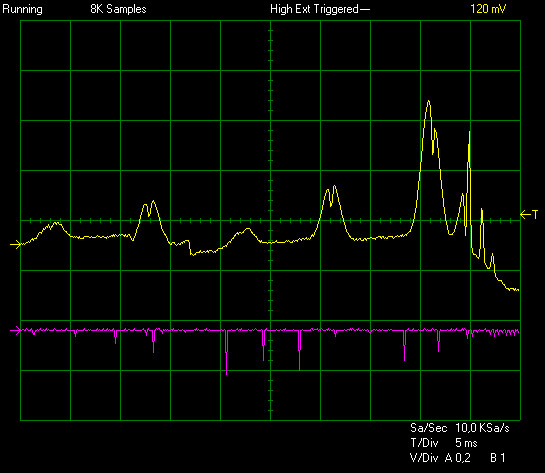
\includegraphics[width=0.3\textwidth]{117mA.jpg}
        \label{fig:figure1}
    }
    \subfigure[$I=118mA$]{
        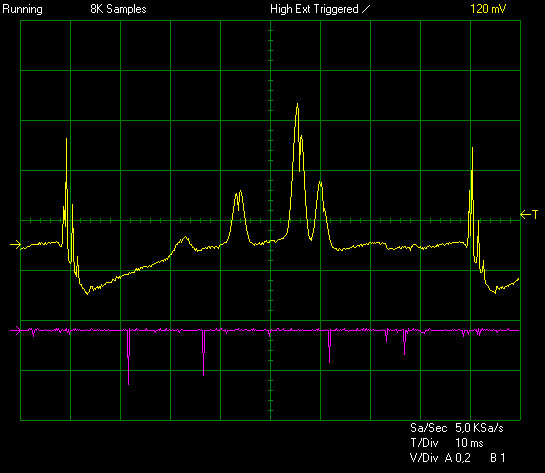
\includegraphics[width=0.3\textwidth]{118mA.jpg}
        \label{fig:figure2}
    }
    \subfigure[$I=119mA$]{
        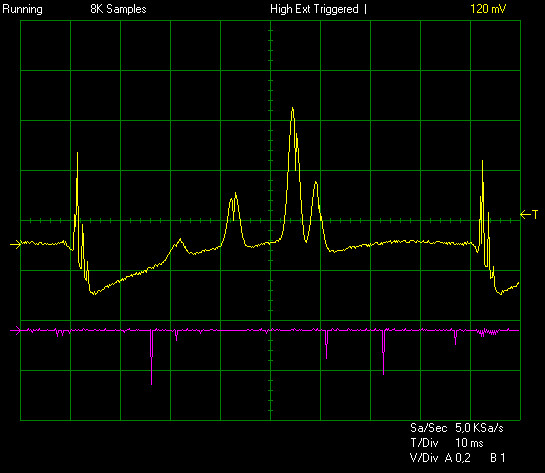
\includegraphics[width=0.3\textwidth]{119mA.jpg}
        \label{fig:figure3}
    }
    \subfigure[$I=120mA$]{
        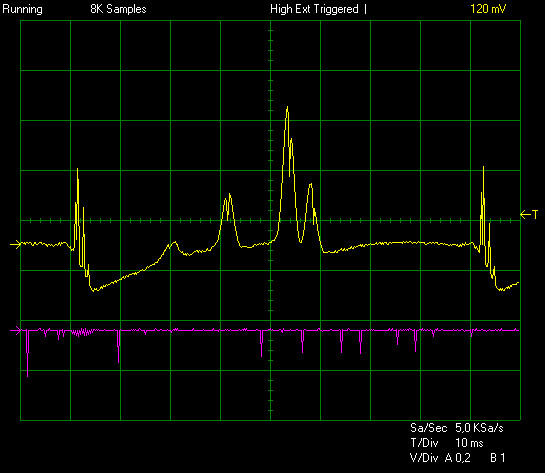
\includegraphics[width=0.3\textwidth]{120mA.jpg}
        \label{fig:figure4}
    }
    \subfigure[$I=121mA$]{
        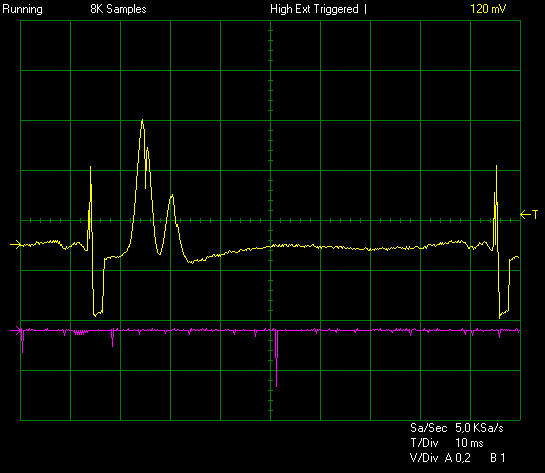
\includegraphics[width=0.3\textwidth]{121mA.jpg}
        \label{fig:figure5}
    }
    \subfigure[$I=122mA$]{
        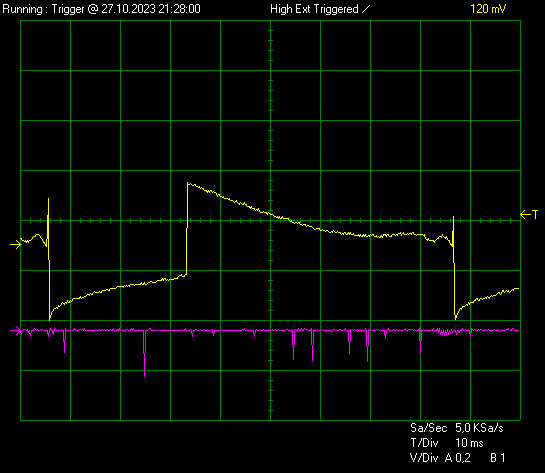
\includegraphics[width=0.3\textwidth]{122mA.jpg}
    }
    \caption{Saturation spectra for variation of injection currents}
    \label{fig:subfigures}
\end{figure}

For the case of constant injection current, a mode jump occurs between $T = \SI{19.9}{\celsius}$ and $T = \SI{20.1}{\celsius}$. We notice that changing the current affects the spectrum more drastically. This could be due to the fact that a slight change in the current leads to more heating compared to the temperature increments we used. 




\begin{figure}[H]
    \centering
    \subfigure[$T = \SI{19.8}{\celsius}$]{
        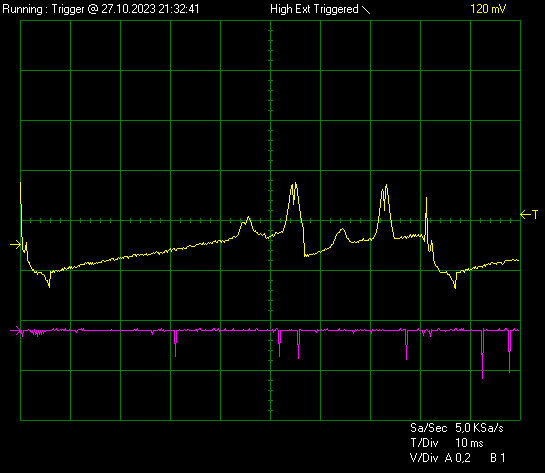
\includegraphics[width=0.3\textwidth]{2/198.jpg}
        \label{fig:figure1}
    }
    \subfigure[$T = \SI{19.9}{\celsius}$]{
        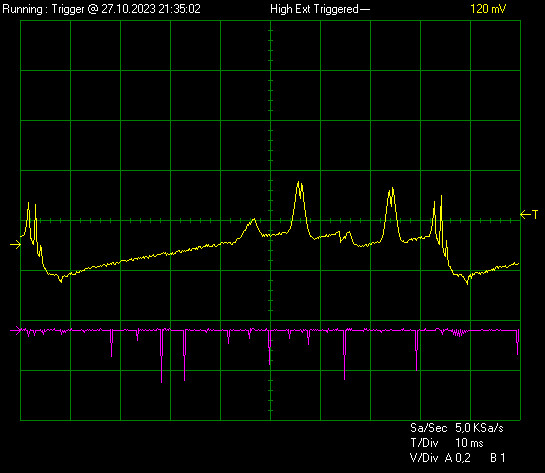
\includegraphics[width=0.3\textwidth]{2/199.jpg}
        \label{fig:figure2}
    }
    \subfigure[$T = \SI{20.1}{\celsius}$]{
        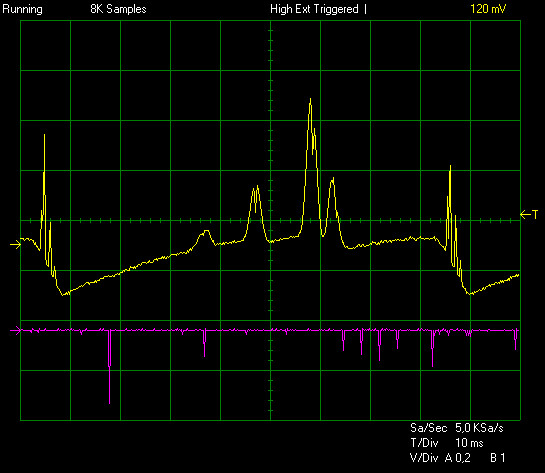
\includegraphics[width=0.3\textwidth]{2/201.jpg}
        \label{fig:figure3}
    }
    \subfigure[$T = \SI{20.2}{\celsius}$]{
        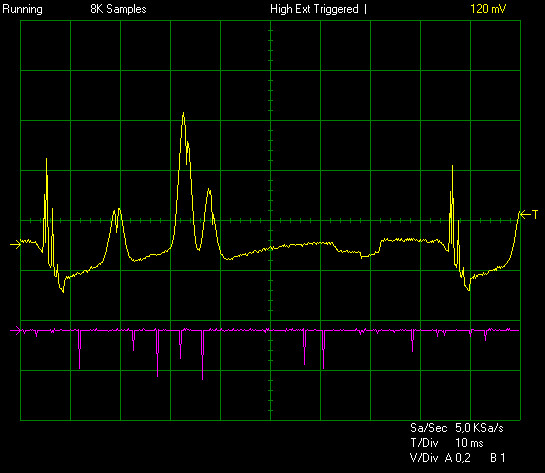
\includegraphics[width=0.3\textwidth]{2/202.jpg}
        \label{fig:figure4}
    }
    \subfigure[$T = \SI{20.3}{\celsius}$]{
        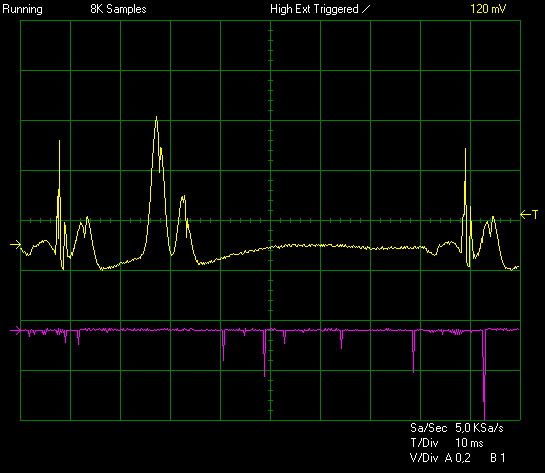
\includegraphics[width=0.3\textwidth]{2/203.jpg}
        \label{fig:figure5}
    }
    \caption{Saturation spectra for variation of temperature}
    \label{fig:subfigures}
\end{figure}

\section{Task 3}
In this task, we consider the effect of replacing the regular filter with a gradient filter at different orientations. We show the saturation spectra we obtained at different angles of the filter. 

\begin{figure}[H]
    \centering
    \subfigure[$\theta = \SI{0}{\degree}$]{
        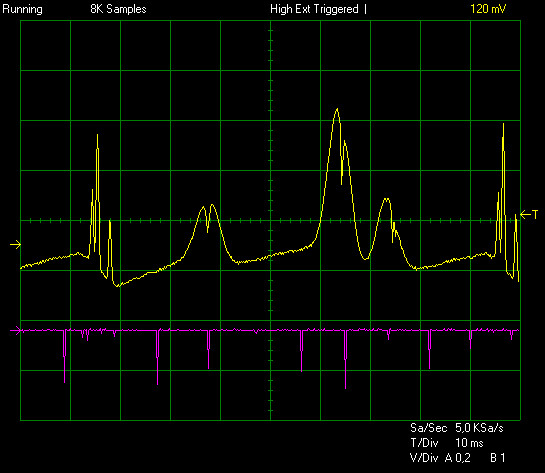
\includegraphics[width=0.3\textwidth]{3/0deg.jpg}
        \label{fig:figure0}
    }
    \subfigure[$\theta = \SI{45}{\degree}$]{
        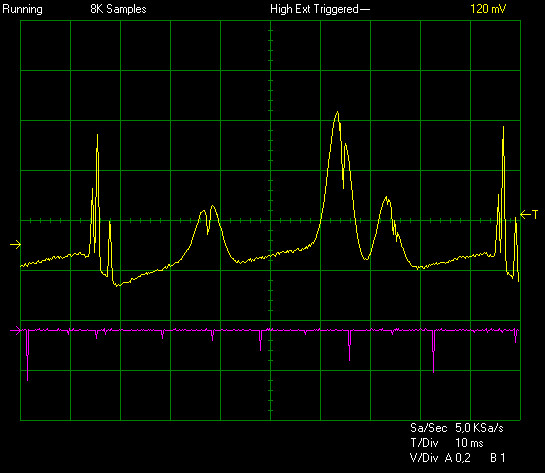
\includegraphics[width=0.3\textwidth]{3/45deg.jpg}
        \label{fig:figure45}
    }
    \subfigure[$\theta = \SI{90}{\degree}$]{
        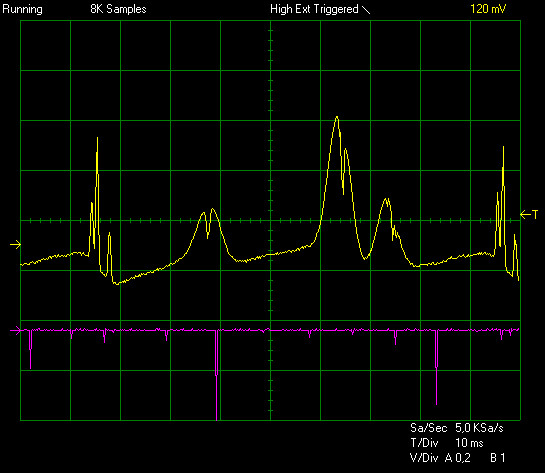
\includegraphics[width=0.3\textwidth]{3/90deg.jpg}
        \label{fig:figure90}
    }
    \subfigure[$\theta = \SI{135}{\degree}$]{
        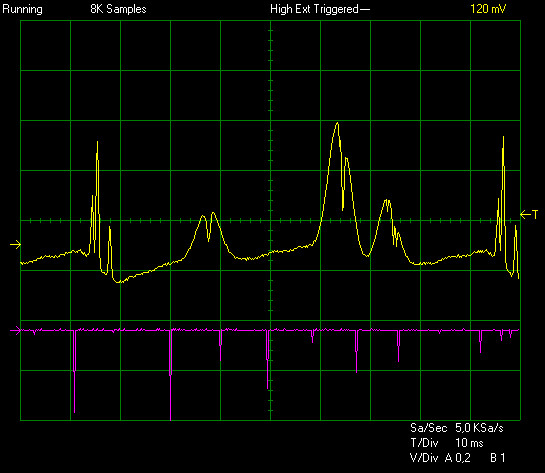
\includegraphics[width=0.3\textwidth]{3/135deg.jpg}
        \label{fig:figure135}
    }
    \subfigure[$\theta = \SI{180}{\degree}$]{
        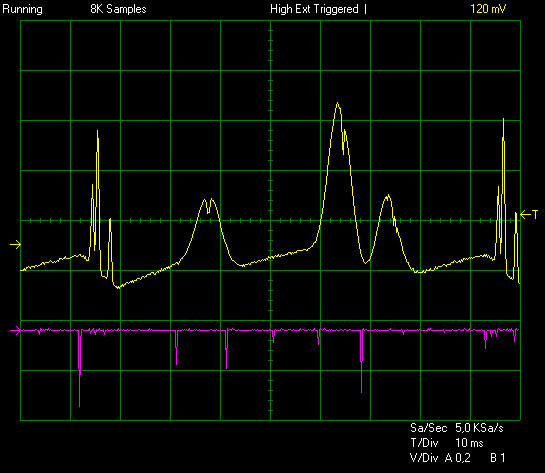
\includegraphics[width=0.3\textwidth]{3/180deg.jpg}
        \label{fig:figure180}
    }
    \subfigure[$\theta = \SI{225}{\degree}$]{
        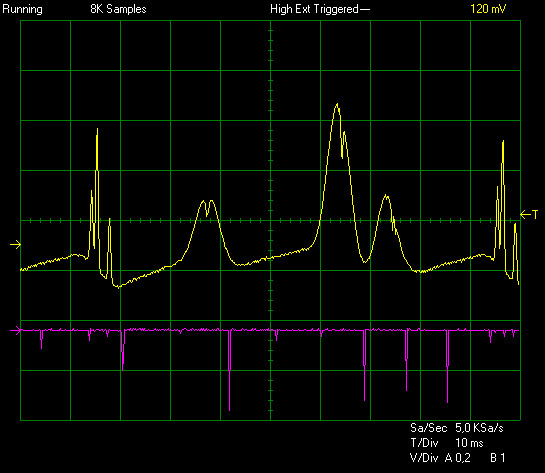
\includegraphics[width=0.3\textwidth]{3/225deg.jpg}
        \label{fig:figure225}
    }
    \subfigure[$\theta = \SI{270}{\degree}$]{
        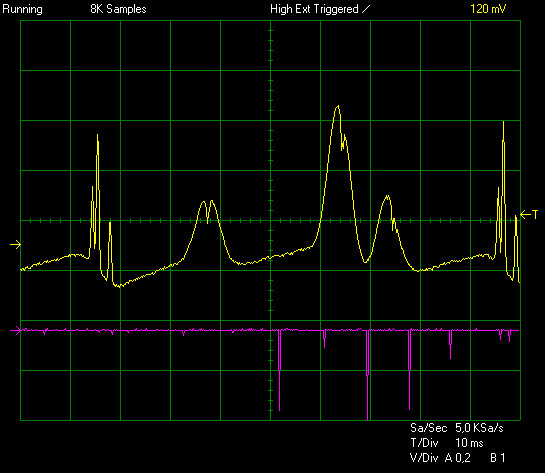
\includegraphics[width=0.3\textwidth]{3/270deg.jpg}
        \label{fig:figure270}
    }
    \subfigure[$\theta = \SI{315}{\degree}$]{
        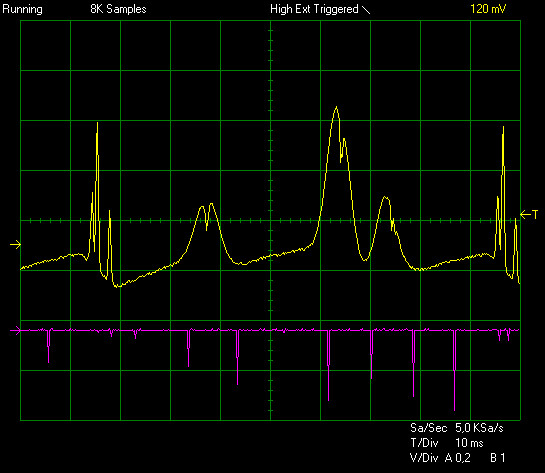
\includegraphics[width=0.3\textwidth]{3/315deg.jpg}
        \label{fig:figure315}
    }
    \subfigure[$\theta = \SI{355}{\degree}$]{
        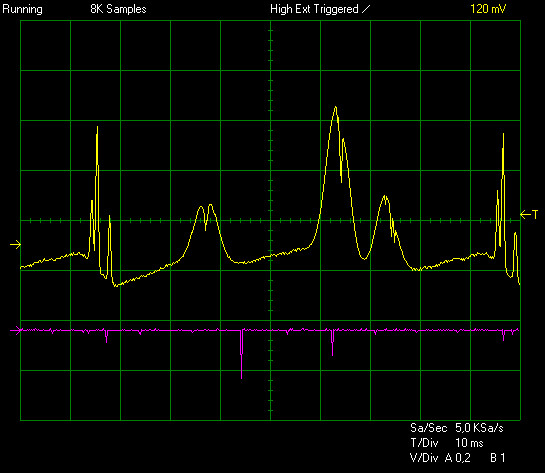
\includegraphics[width=0.3\textwidth]{3/355deg.jpg}
        \label{fig:figure355}
    }
    \caption{Saturation spectra for different angles}
    \label{fig:subfigures}
\end{figure}

The main observation is the decrease of peak heights as the filtering (i.e. the angle $\theta$) increases. No change was observed for the peak positions. This is due to the position of the filter in our setup. The filter only affects the probe beam and not the pump beam. Therefore, the proportion of population inversion stays the same while the intensity of the saturation peaks goes down. Moreover, the FPI peaks were not affected by changing the filtering. This is because the filter is placed after the beam splitter which controls how much of the initial beam goes into the interferometer. At $\theta=\SI{180}{\degree}$ a significant increase is observed. 
\\\\
We also tested another filter which is thicker than the one we used and observed only a change in the intensity while all other aspects stayed invariant. A comparison of the thin vs thick filter is shown in the figure below. The spectrum looks different here because we are zoomed-in to a specific peak (peak 4) from the previous figures. 


\begin{figure}[H]
    \centering
    \subfigure[Thin filter]{
        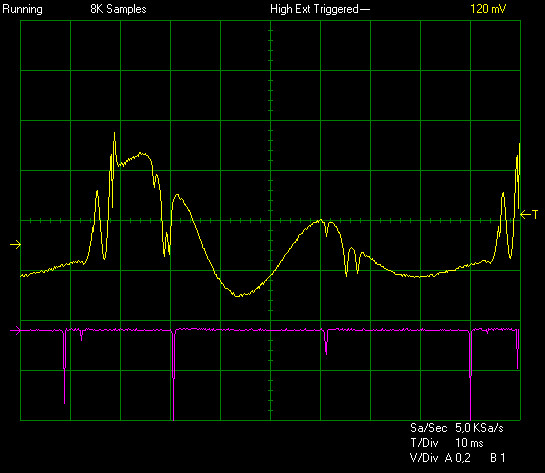
\includegraphics[width=0.3\textwidth]{110ThinFilter.jpg}
        \label{fig:figure0}
    }
    \subfigure[Thick filter]{
        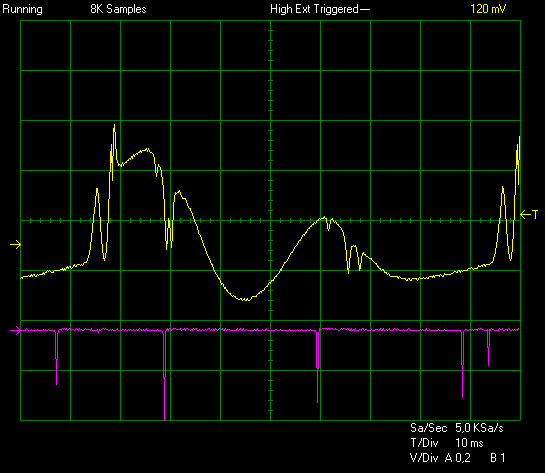
\includegraphics[width=0.3\textwidth]{110ThickFilter.jpg}
        \label{fig:figure45}
    }

\end{figure}













\end{document}


